\subsection{Greedy Heuristics Algorithm}

The general idea in the approach taken in this section, is using Dijkstra's algorithm for finding the shortest path with distance over speed as the weight of an edge. The problem then becomes, which speed must we use in the interval of $v_{min}$ and $v_{max}$. As argued previously, the optimal speed to drive can only be found by iterating over all possibilities which is a combinatorial optimization problem, and it is NP-Hard. Thus we introduce a heuristic, which promotes local optimal choices. This gives a fast path, but this might not be drivable, if there are not any charging stations on this path, thus we will need to figure out how to incorporate this.

We will now analyse how the weight can be found, specifically the speed. The time spent passing an edge $e = (u_1, u_2)$ in the road network, is given by the following equation:

\begin{equation*}
\begin{aligned}
 & T(v,(u_1, u_2)) = \frac{D((u_1, u_2))}{v} + \frac{R_{CO}(v) * D((u_1, u_2)) - B_{cur}}{Best_{CH}(u_1)}
\end{aligned}
\end{equation*}\label{eq:drivingAndCharging}

where $v$ is the speed of the vehicle, $D(u_1, u_2)$ is the distance between vertices $u_1$ and $u_2$, $R_{CO}(v)$ is the consumption rate of the vehicle at the speed $v$, $B_{cur}$ is the current battery capacity of the vehicle 
and $Best_{CH}(u_1)$ is the charge rate of the best charging station previous to $u_1$ or the charge rate of $u_1$.

The above equation yields a function on the form: $av^2 + bv + c$, due to the fact that 
$R_{CO}(v)$ is a quadratic function. $a$ , $b$ and $c$ are some constants which are given by the instance of the vehicle. 
Represented in a Cartesian coordinate system, $T(v,(u_1, u_2)))$ is a parabola, as can be seen in \Cref{fig:graph}. On the x-axis is the speed of the vehicle and on the y-axis is the time spent. The turning point of the graph represents the optimal speed to drive at for the given edge, denoted as $v_{opt}(e)$. The point is easily calculated by finding a tangent line with a slope of $0$. If $v_{opt}(e)$ is smaller than $v_{min}(e)$, then $v_{min}(e)$ defines the optimal speed for the edge. Similarly if $v_{opt}(e)$ is larger than $v_{max}(e)$, $v_{max}(e)$ defines the optimal speed for the edge.

The time spent driving an edge $(u_1, u_2)$, using the energy in the battery, can be found by solving:
\[B_{cur} - D(u_1, u_2) * R_{CO}(v) = 0\] 
if $v_{opt}(e)$ is lower than $v_{min}(e)$ the time used driving is set to infinity, since there is not enough energy in the battery to drive from $u_1$ to $u_2$. Otherwise $v_{opt}$ is decided in the same way when charging is considered.

\begin{figure}[!htb]
\label{fig:graph}
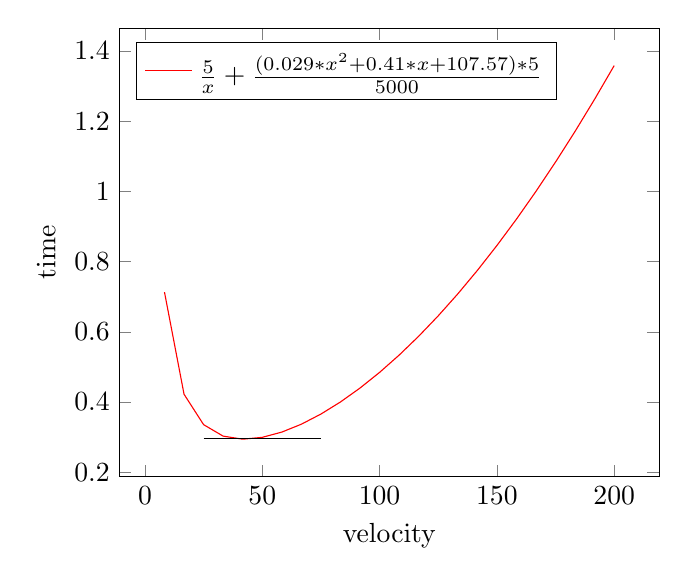
\begin{tikzpicture}
\begin{axis}[xlabel=velocity, ylabel=time,legend style={legend pos=north west}]
\addplot[draw=red,domain=0:200]{(5/x)+(((0.0286*x^2 + 0.4096*x + 107.57)*5)/5000)};
\addlegendentry{$\frac{5}{x}+\frac{(0.029*x^2 + 0.41*x + 107.57)*5}{5000}$}

\addplot[draw=black,domain=25:75]{0.295};
% \addplot[mark=*, domain=25:75] coordinates {(37,295)};
\end{axis}
\end{tikzpicture}% 
\caption{In this instance of $T(v,(u_1, u_2))$, going from $u_1$ to $u_2$, we have a distance of $5 \si{\km}$ and a charge speed of $5 \si{\kW}$ on $u_1$. The optimal speed in this case is $42.12\si{\miles\per\hour}$, which takes roughly 7 minutes to drive}
\end{figure}

The above can be used to create a function, which help us find the optimal way to drive a road segment. 

\[travel\_time(charge\_stations, (u_1, u_2), B_{cur}) \]

we have a way of deciding the time it will take to drive a road segment, while accounting for the need of charging along the path. This function is used with Dijkstra's algorithm where we use the time instead of distance. Just like Dijkstra's algorithm we keep track of the fastest path leading to each vertices, where shortest path in turn means the path using least time. Furthermore all previous charging stations on the current path, that are within range and still can be used for charging, needs to be stored on each vertex. This way we will charge at a station after leaving it, if we do not violate the physical constraints in the system(i.e. no over-charging). Lastly the algorithm need also to keep track of how much battery the EV have, when it first arrives at a charging station.

While the algorithm progresses through the graph, it need to store a subset of the charging stations on the current path. At every reached charging station, we record the possible energy$B_{possible}$ we can add to the system, defined by $B_{cap}-B_{cur}$ and the charge rate of the station as a tuple: $(B_{possible}, R_{CH}(vertex))$.

We maintain a subset of tuples on every vertex by using a list of tuples only with $B_{possible}$ above 0. This will of course always be the case when we reach a charging station, but as we progress through the graph and some distance is being traveled, the possible energy at each previous charging station decreses. The first tuple in the list will always be the the charging station with the best charge rate. A tuple is removed either when $B_{possible}$ hit 0, or when new tuple, with a higher charge rate is found. We make sure to store the best charging station at position 0 in the list, by remove every tuple between the first and second best charge rate in the list. Using this we can define a fastest path algorithm in the following way: 

\begin{algorithmic}
\Function{fastestPath}{$G,s,t$}
	\ForAll{$v \in G.V$} 
    		\State $v.time = infinity$
		\State $v.path = [v]$
    		\State $v.preCH = []$
		\State $v.myCH = [batCap, v.charge\_speed]$
		\State $v.B_{cur} = 0$
    	\EndFor
	\State $s.time = 0$
	\State $s.B_{cur} = initialBattery$
	\State $s.preCS.append(s)$	
	\State $Q = G.V sorted by time$
	\While{Q} 
		\State $u = Q[0]$
		\State $Q.remove[u]$
		\If{$u.time == infinity$} break \EndIf
		\ForAll{$adj(u)$} 
			\State $travel = travel\_time(u.preCS, (u, v), B_{cur})$
			\State $time = travel[1]$
			\State $preCH = travel[2]$
			\State $curbat = travel[3]$
			\If{t$ime == infinity$} break \EndIf
			\If{$v.time > u.time + time$} 
				\State $v.time = u.time + time$
				\State $v.path = u.path + [v]$
				\State $v.B_{cur} = curbat$
				\State $v.preCS = cleanCS(preCS, u, curbat)$
				\State reposition $v$ in $Q$
			\EndIf

		\EndFor
	\EndWhile
	\State \Return $t.time, t.path$
\EndFunction
\end{algorithmic}\label{alg:fastest_path}
\todo[inline]{hvor bliver den bedste charging station valgt?\\
hvor bliver charging stations ryde op?}
